\begin{comment}
\section{Osservabili stellari/demo beamer}
\begin{frame}<1>[label=noinside]{Modello stellare}{Come indagare la fisica interna a una stella?}
\onslide<1->\begin{block}{Osservabili stellari:}
$L$, $M$, $R$, $T_e$, $(\frac{Z}{X})_{ph}$, $g_{ph}$.
\end{block}
\onslide<1->\begin{block}{Informazioni sulla struttura interna?} Condizione di equilibrio idrostatico
\end{block}
%Teorema Vogt-Russel: $X_i(r)$, $M$ \pause equilibrio (idrostatico/termico) determinano struttura stellare .
%\pause
\onslide<1->\begin{block}{Modello stellare: diagramma di \hr{}.}
\end{block}
\onslide<2->\begin{block}{Descrizione fisica interno stellare: parametri aggiuntivi}
Convezione, diffusione e sedimentazione elementi pesanti, equazione di stato, opacit\'a
\end{block}
\onslide<2->\begin{block}{Astrosismologia}
Restringo spazio parametri sistemi stellari lontani
\end{block}
\end{frame}
{ % all template changes are local to this group.
    \setbeamertemplate{navigation symbols}{}
    \begin{frame}[plain]{Diagramma di \hr{}}
        \begin{tikzpicture}[remember picture,overlay]
            \node[at=(current page.center)] {
                %\includegraphics[width=\paperwidth]{yourimage}
            };
        \end{tikzpicture}
     \end{frame}
}
\againframe<2>{noinside}
\begin{frame}{Pulsazioni stellari}{Modi Normali}
\begin{columns}
\begin{column}{0.5\textwidth}  %%<--- here
    \begin{center}
     %\includegraphics[width=0.5\textwidth]{image1}
     \end{center}
\end{column}
\begin{column}{0.5\textwidth}
\onslide<1-> \begin{block}{Stelle pulsanti}
Onde stazionarie: Pulsazione radiale/non radiale: .
\onslide<2-> meccanismo di eccitazione: solar-like pulsator, Cefeidi.
\onslide<3-> Modo fondamentale $\Pi\approx\tau_{dyn}=\sqrt{\frac{R^3}{GM}}\propto\overline{\rho}\expy{-\frac{1}{2}}$.
\onslide<4-> Modi di oscillazione\onslide<5-> - informazioni sull'interno stellare
\onslide<5-> Elio-sismologia: Modi $\Leftrightarrow$ Modelli solari
\onslide<5-> Astero-sismologia: Modi $\Leftrightarrow$ Spazio parametri modello stellare
\end{block}
\end{column}
\end{columns}
\end{frame}

\end{comment}

\section{Osservabili solari}

\begin{frame}{Dati osservativi}

\begin{block}{Et\'a, luminosit\'a, raggio solari}
\begin{tabular}{l|c}
\hline
$\agesun{}$&\SI[separate-uncertainty=true]{4.57\pm0.02e9}{\year}\\
\hline
$\rsun{}$&\SI{695658+-140}{\kilo\meter}\\
\hline
$G\msun$&\num{132712440018+-8}\SI{e9}{\cubic\meter\per\square\second}\\
\hline
$\lsun{}$&\SI{3.8275+-0.0014e33}{\erg\per\second}\\
\hline
\end{tabular}
%\caption[Osservabili solari principali.]{Osservabili solari principali. \cite{haberreiter2008solving}.}
\label{tab:sunO}
\end{block}

\begin{block}{Simmetria sferica}
Deviazioni da forma sferica trascurabili (campi magnetici, rotazione)
\end{block}

\end{frame}

\begin{frame}{Dati osservativi}

\begin{block}{Composizione chimica}
\begin{itemize}
\item Righe di assorbimento: attuale (non $Y_{ph}$)
\item Meteoriti CI: primordiale (refrattari)
\end{itemize}

\begin{table}[]

\pgfplotstabletypeset[
every head row/.style={
 before row={\toprule &\multicolumn{4}{c|}{Attuale}
 %&\multicolumn{4}{c|}{Primordiale}
 \\\midrule},
 every last row/.style={after row=\bottomrule},
 after row={\midrule}
},
every nth row={2}{before row=\midrule},every last row/.style={after row=\bottomrule},
every first column/.style={column type/.add={|}{}},
every last column/.style={column type/.add={}{|}},
columns/x/.style = {column type/.add={|}{}},
columns/xi/.style = {column type/.add={|}{}},
display columns/0/.style={column name={}},
display columns/1/.style={column name={$X$}},
display columns/2/.style={column name={$Y$}},
display columns/3/.style={column name={$Z$}},
display columns/4/.style={column name={$\frac{Z}{X}$}},
%display columns/5/.style={column name={$X$}},
%display columns/6/.style={column name={$Y$}},
%display columns/7/.style={column name={$Z$}},
%display columns/8/.style={column name={$\frac{Z}{X}$}},
create on use/authors/.style={create col/set list={
%Anders \& Grevesse (1989),Grevesse \& Noels (1993),
Grevesse et al. (1998),Lodders (2003),Asplund et al. (2005),Lodders et al. (2009),\cite{asplund2009chemical},\cite{caffau2011solar}}},
columns/authors/.style={string type},
columns={authors,x, y, z, zx
%,xi,yi,zi, zxi
},
/pgf/number format/precision=4
     ]{asplund.txt} %%%
\captionof{table}{Metallicit\'a attuale determinata da varii autori.}\label{tab:Zhistory}
\end{table}

\end{block}

\end{frame}


\section{Strutture autogravitanti in equilibrio}

\begin{frame}{Distribuzione di massa - Conservazione di massa e momento - tempo scala dinamico}

\begin{block}{Massa}

%\begin{align}
%&dm=4\pi r^2\rho \,dr-4\pi r^2\rho v\,dt\label{eq:massvar}\\
%\end{align}

\begin{equation}
\PDy{t}{\rho}+\nabla\cdot(\rho\vec{v})=0\label{eq:continuityeq}
\end{equation}

\begin{equation}
dm=4\pi r^2\rho \,dr\label{eq:massaguscio}
\end{equation}

\end{block}

\begin{block}{Momento}
\begin{align}
&\rho\TDy{t}{\vec{v}}=-\nabla P+\rho\vec{f}\label{eq:motion}\\
&\vec{g}=-\PDy{r}{\Phi}=-\frac{Gm(r)}{r^2}\hat{r}
\end{align}
\end{block}

\end{frame}

\begin{frame}{Equilibrio idrostatico: $\ddvec{r}=0$.}

\begin{align}
\nabla P=\rho \vec{f}\Label{eq:idrosta} \TDy{r}{P}=-\frac{Gm(r)\rho(r)}{r^2}\Label{eq:fidroequilibrio}
\end{align}


Per giustificare l'ipotesi di equilibrio idrostatico stimo i tempi caratteristici di evoluzione della struttura solare nel caso la forza dovuta alla pressione o la forza di gravit\'a non fossero bilanciate, approssimando il valore caratteristico della derivata di due variabili con il rapporto del loro valore caratteristico.

\begin{equation}
\tau_{ff}\approx\tau_{esp}\approx\tau_{idro}^{\odot}= \sqrt{\frac{R^3}{GM}}\approx\frac{1}{2}(G\overline{\rho})\expy{-\frac{1}{2}}\approx\SI{27}{\minute}
\end{equation}

\end{frame}

\subsection{Equazione di stato $P(\rho,T)$}

\begin{frame}{Gas perfetto ioni-elettroni}


\begin{equation}
P_G=P_I+P_e=\frac{\rho}{\mu}\gasconstant{}T
\end{equation}

\begin{block}{Peso molecolare medio}
massa media in amu per particella libera
\begin{align}
&\mu=\frac{1}{\bar{n}_HX+\bar{n}_{He}Y+\bar{n}_{Z}Z}\label{eq:meanmw}\\
&\bar{n}_i=\frac{1+f_i}{A_i}
\end{align}

\end{block}


\end{frame}

\subsection{Energia interna per unit\'a di massa}

\begin{frame}{Energia interna: traslazioni}

\begin{align}
&u=\frac{1}{\rho}\sum_i\int f^{(0)}(\vec{p}_i)\frac{p^2_i}{2m_i}=\frac{3}{2}\frac{P}{\rho}=\frac{3}{2}\frac{\gasconstant T}{\mu}\\
&E_i=\int_0^Mu\,dm=\frac{3}{2}\int_M\frac{P}{\rho}\,dm\label{eq:traslintenergy}
\end{align}

 $f^{(0)}(\vec{p}_i)$ \'e il numero di particelle della specie i per unit\'a di volume con impulso in $[\vec{p},\vec{p}+d\vec{p}]$

\end{frame}


\subsection{Correzioni alla legge dei gas perfetti}

\begin{frame}{Correzioni alla legge dei gas perfetti}

\begin{itemize}
\item Degenerazione elettronica ($\Delta P\leq2\%$).

\begin{align}
&P_{FD}=[\exp{\psi(\rho,T)+\midfrac{p^2}{2mKT}}+1]\expy{-1}\\
&n_e=\frac{\rho N_A}{\mu_e}=\frac{8\pi}{3h^3m_e}(2m_eKT)\expy{\midfrac{3}{2}}F_{\midfrac{3}{2}}(\psi(\rho,T))\\
%n_e=\intzi{}\frac{8\pi p^2\,dp}{h^3(\exp{\frac{u_k}{KT}-\psi}+1)}\\
&P_e=\frac{1}{3}\intzi{}pn_e\TDy{p}{u_k}\,dp
\end{align}

\item Pressione di radiazione: $P_r=\frac{1}{3}aT^4$.

\item Ionizzazione.

\end{itemize}

\end{frame}

\begin{frame}{Correzioni alla legge dei gas perfetti: Interazioni coulombiane}

\begin{align}
&\frac{1}{r_D^2}=\frac{4\pi e^2}{kT}\sum Z^2\overline{n}_Z=\frac{4\pi e^2}{kT}N_A\zeta\\
&\zeta=\sum_{i}(Z_i^2+Z_i)\frac{\rho X_i}{A_i}\xrightarrow{FD}\sum_{i}(Z_i^2+\frac{F_{\midfrac{3}{2}}'(\psi)}{F_{\midfrac{3}{2}}(\psi)}_i)\frac{\rho X_i}{A_i}
\end{align}

\begin{equation}
u_c=\frac{1}{2}\int\phi(\vec{r})\rho_c(\vec{r})\,d^3r,\ P_c=\frac{1}{3}u_c
\end{equation}

Regioni di ionizzazione parziale di idrogeno ed elio

\end{frame}

\begin{frame}{EOS}

\begin{itemize}
\item Schema chimico (MHD): atomi e molecole, stati eccitati e diversi gradi di ionizzazione

\item Schema fisico (OPAL): nuclei ed elettroni, potenziale Coulombiano, Schr\"oedinger per un problema a molti corpi.
\end{itemize}

\begin{figure}[!ht]
\subfigure[Popolazione dei diversi gradi di ionizzazione per $\cel{He}{4}{}{}$, CNO, $\cel{Ne}{20}{}{}$, $\cel{Fe}{56}{}{}$. Da \cite{basu2008helioseismology}.]{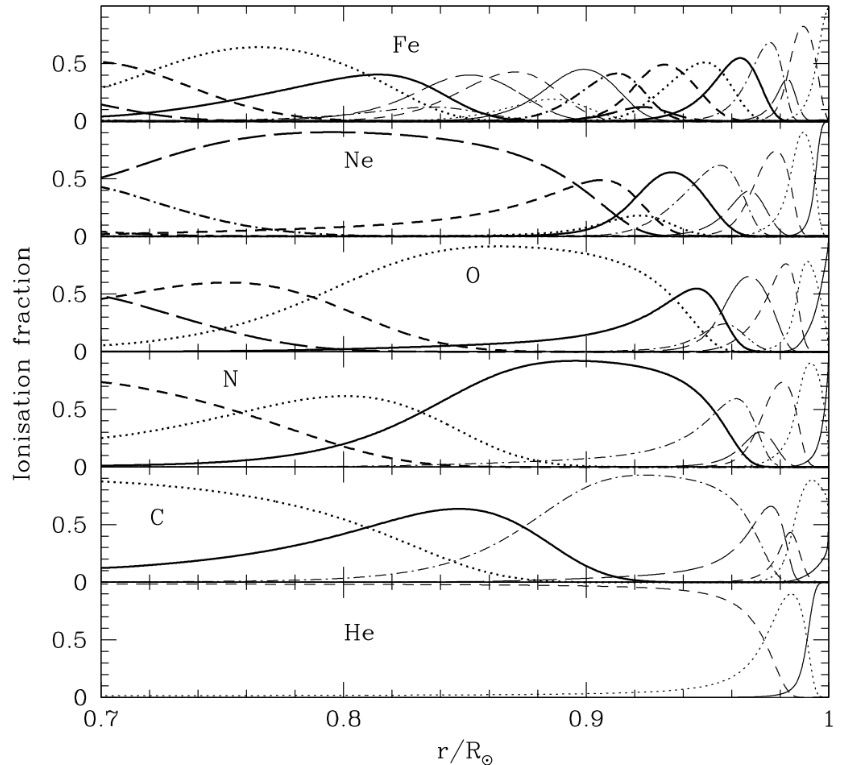
\includegraphics[width=0.4\textwidth,keepaspectratio]{ionfraction}}\label{ionfraction}
%\subcaption{Andamento di $\Gamma_1$ calcolato tramite equazione di stato MHD/OPAL. Da \cite{trampedach2006synoptic}.]{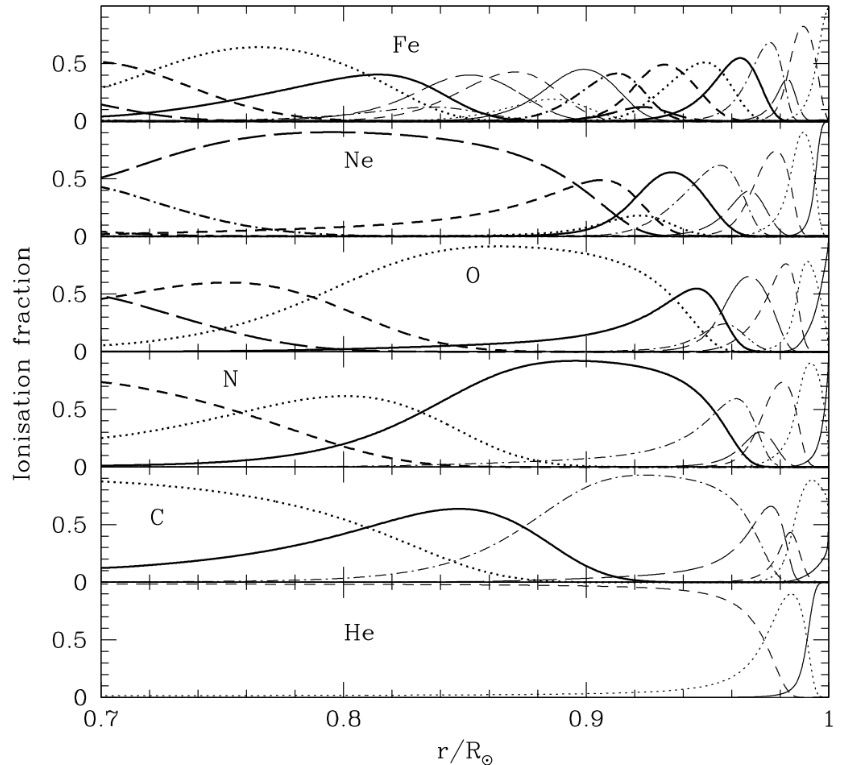
\includegraphics[width=0.4\textwidth,keepaspectratio]{ionfraction}}
~
\subfigure[Confronto $\Gamma_1$ MHD/OPAL. Da \cite{trampedach2006synoptic}.]{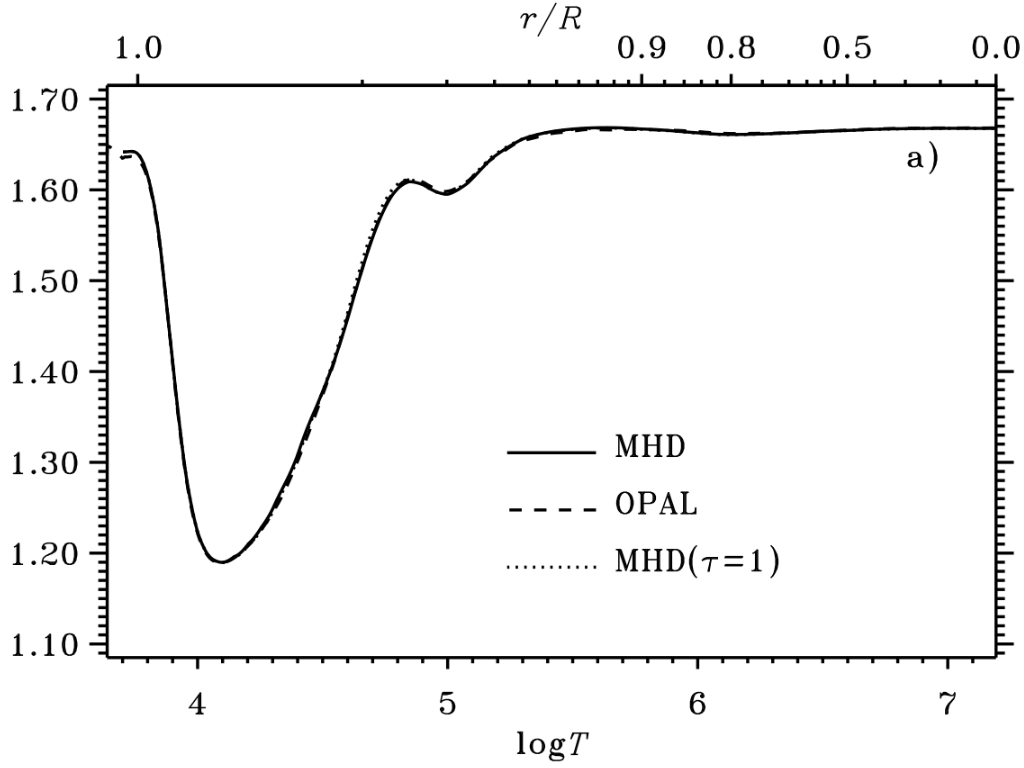
\includegraphics[width=0.4\textwidth,keepaspectratio]{gamma1eos}}
%\subcaption{Profilo radiale della popolazione dei diversi gradi di ionizzazione per $\cel{He}{4}{}{}$, CNO, $\cel{Ne}{20}{}{}$, $\cel{Fe}{56}{}{}$. Stati di ionizzazione maggiore sono pi\'u interni. Da \cite{basu2008helioseismology}.}\label{ionfraction}
%\subcaption{Andamento di $\Gamma_1$ calcolato tramite equazione di stato MHD/OPAL. Da \cite{trampedach2006synoptic}.}\label{fig:gamma1eos}
\end{figure}


\end{frame}


\section{Trasporto dell'energia}

\subsection{Teorema del viriale}

\begin{frame}{T Viriale}

Il teorema del viriale esprime una propriet\'a statistica di particelle interagenti: 

L'energia potenziale gravitazionale della stella \'e
\begin{equation}
\Omega=-\int_0^M\frac{Gm(r)}{r}\,dm\label{eq:energiapg}
\end{equation}

\begin{equation}
\frac{1}{2}\TtwoDy{t}{I}=2E_i+\Omega
\end{equation}
con $E_i$ data da \eqref{eq:traslintenergy} e $I=\int r^2\,dm$. In condizioni stazionarie $\frac{1}{2}\TtwoDy{t}{I}\approx0$:
\begin{equation}
0=\int_M\frac{3P}{\rho}\,dm(r)+\Omega
\end{equation}

Detta $W=E_i+\Omega$ l'energia totale della stella, si ha:
\begin{equation}
\Omega=-2E_i\label{eq:virialegpm}
\end{equation}
e dalla conservazione dell'energia $\TDy{t}{W}+L=0$ segue che durante la fase di collasso prima dell'inizio della sequenza principale met\'a dell'energia gravitazionale viene spesa per aumentare l'energia interna e met\'a in luminosit\'a:
\begin{equation}
L=-\frac{1}{2}\dot{\Omega}=\dot{E}_i
\end{equation}

\subsection{Struttura in equilibrio idrostatico e termico in assenza di reazioni nucleari}

Nel caso in cui la contrazione gravitazionale sia l'unica fonte di energia per una massa gassosa in equilibrio idrostatico, il suo tempo di evoluzione caratteristico \'e il tempo di \kh{}:
\begin{equation}
\tkh{}=\frac{\Omega}{L}\approx\frac{GM^2}{2RL}\approx\SI{1.6e7}{\year}
\end{equation}

cammino libero medio degli atomi e dei fotoni sia breve, si raggiunge rapidamente l'equilibrio idrostatico e termico locale. Il processo di contrazione gravitazionale continua, su tempi-scala termodinamici, fino a che l'energia prodotta dalle reazioni nucleari bilancia l'energia irradiata.


\end{frame}


\subsection{Conservazione dell'energia interna}

\begin{frame}{Prima legge TD}

$dq$ per unit\'a di massa per $dt$:
\begin{align}
&\TDy{t}{q}=\TDy{t}{u}+P\TDof{t}(\frac{1}{\rho})\label{eq:prima}\\
%\TDy{t}{u}+P\TDy{t}{V}
&\TDy{t}{\ln{T}}=\frac{\Gamma_2-1}{\Gamma_2}\TDy{t}{\ln{P}}+\frac{\TDy{t}{q}}{c_PT}\label{eq:primatemp}\\
&\TDy{t}{\ln{P}}=\Gamma_1\TDy{t}{\ln{\rho}}+\frac{\rho(\Gamma_3-1)}{P}\TDy{t}{q}\label{eq:primapres}
\end{align}
Esponenti adiabatici $\Gamma_i$:
\begin{equation}\label{eq:adibatexp}
\Gamma_1=\Dcvar{\TDly{\rho}{P}}{Ad}, \ \Gamma_3-1=\Dcvar{\TDly{\rho}{T}}{Ad},\ \frac{\Gamma_2-1}{\Gamma_2}=\Dcvar{\TDly{P}{T}}{Ad}
\end{equation}

\end{frame}

\section{Equilibrio termico}

\begin{frame}{Equilibrio termico}

Scrivo il bilancio di calore per un elemento di massa unitaria di gas:
\begin{equation}
\TDy{t}{q}=\epsilon-\frac{1}{\rho}\nabla\cdot\vec{F}\label{eq:heatgl}
\end{equation}
dove $\epsilon$ \'e l'energia prodotta per unit\'a di tempo e massa e $\vec{F}$ \'e il flusso di energia verso l'esterno generalmente dovuto alla diffusione di fotoni dalla zona pi\'u calda verso la superficie; sostituendo in \eqref{eq:prima} si ha
\begin{equation}
\TDy{r}{L}=4\pi r^2[\rho\epsilon-\rho\TDof{t}u+\frac{P}{\rho}\TDy{t}{\rho}]\label{eq:fenergyconservation}
\end{equation}

Nel caso stazionario:
\begin{equation}
\TDy{t}{q}=0\ \Rightarrow\ dL=4\pi r^2\rho\epsilon\,dr
\end{equation}
e i processi nucleari che avvengono nella parte centrale forniscono il calore per bilanciare il flusso di energia irradiata.


\end{frame}


\section{Produzione di energia - reazioni di fusione}

\begin{block}{Schermaggio debole: $e\phi\ll KT$.}



\end{block}

\section{Modello solare standard e osservabili sismologiche}


